\documentclass{beamer}

\usepackage{graphicx, tikz}

\title{My fantastic presentation}
\author{Firstname Lastname}
\institute{University of Puuhamaa}
\titlegraphic{\includegraphics[width=3cm]{../pictures/TheDogs.jpg}}
\date{20 May 2024}

\begin{document}

\maketitle


\begin{frame}
\frametitle{Hi there!}

Welcome to my presentation!

We will talk about Pythagoras and his theorem.
\end{frame}


\begin{frame}
\frametitle{Hi there!}

Welcome to my presentation!

\begin{block}{Goal}
You will learn about Pythagoras and his theorem.
\end{block}
\end{frame}


\begin{frame}
\frametitle{The theorem}

\begin{theorem}
If $a$ and $b$ are the lengths of catheti of a right-angled triangle,
then the hypothenuse has length $\sqrt{a^2 + b^2}$.
\end{theorem}
\begin{proof}
We'll get to this soon.
\end{proof}

\end{frame}


\begin{frame}
\frametitle{Comparison of Pythagoras and his theorem}

\begin{columns}
\begin{column}{0.5\textwidth}

Properties of \alert{Pythagoras}:
\begin{enumerate}[1.]
    \item From Ancient Greece
    \item Three-dimensional
    \item Historical facts unknown
\end{enumerate}

\end{column}

\begin{column}{0.5\textwidth}

Properties of \alert{the theorem}:
\begin{enumerate}[i)]
    \item Not invented by Pythagoras
    \item Two-dimensional
    \item A mathematical fact
\end{enumerate}

\end{column}
\end{columns}

\end{frame}


\begin{frame}
\frametitle{Some pictures}

\begin{figure}
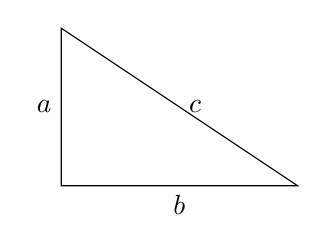
\begin{tikzpicture}

\draw (0,0) -- (0,2) node[pos=0.5, left] {$a$}
    -- (3,0) node[pos=0.5, right] {$c$}
    -- cycle node[pos=0.5, below] {$b$};

\end{tikzpicture}
\caption{A right triangle.}
\end{figure}

\begin{figure}
\includegraphics[width=3cm]{../pictures/TheDogs.jpg}
\caption{Slide hijacked by a dog!}
\end{figure}

\end{frame}


\begin{frame}
\frametitle{A digression on numbers}

\begin{theorem}
Every natural number has a successor.
\end{theorem}

\pause

\begin{theorem}
There is at least one natural number.
\end{theorem}

\pause

\begin{corollary}
There are infinitely many natural numbers.
\end{corollary}

\end{frame}


\begin{frame}
\frametitle{On the infinitude of numbers}

\begin{corollary}
There are infinitely many natural numbers.
\end{corollary}
\begin{proof}
\uncover<2->{Suppose that $n$ is the largest natural number.}
\uncover<3->{But then its successor $n+1$ is an even larger natural number.}
\end{proof}

\end{frame}


\begin{frame}

\textbf<1>{Bold on the first slide only.}\\
\alert<2>{Alerted on the second slide only.}

\end{frame}


\begin{frame}

There is nothing to see here.\\
\only<2>{\includegraphics[width=6cm]{../pictures/TheDogs.jpg}\\}
Absolutely nothing at all.

\end{frame}


\end{document}
